\section{The Agent Harness: Enacting Grounding}

The Agent Harness is the runtime architecture that bridges the LLM's frozen prior (\(\mathcal{K}\), L1--L3) with real-time L4 states. It supplies observation, belief update, and execution. The LLM provides the prior and approximates planning; the Harness closes the loop. Grounding is an emergent property of the coupled system, not of the model alone.
% 智能体框架是连接LLM冻结先验（\(\mathcal{K}\)，L1-L3）与实时L4状态的运行时架构。它提供观测、信念更新和执行。LLM提供先验并近似规划；框架闭合环路。落地是耦合系统的涌现属性，而非模型单独的性质。

\begin{figure*}[t]
    \centering
    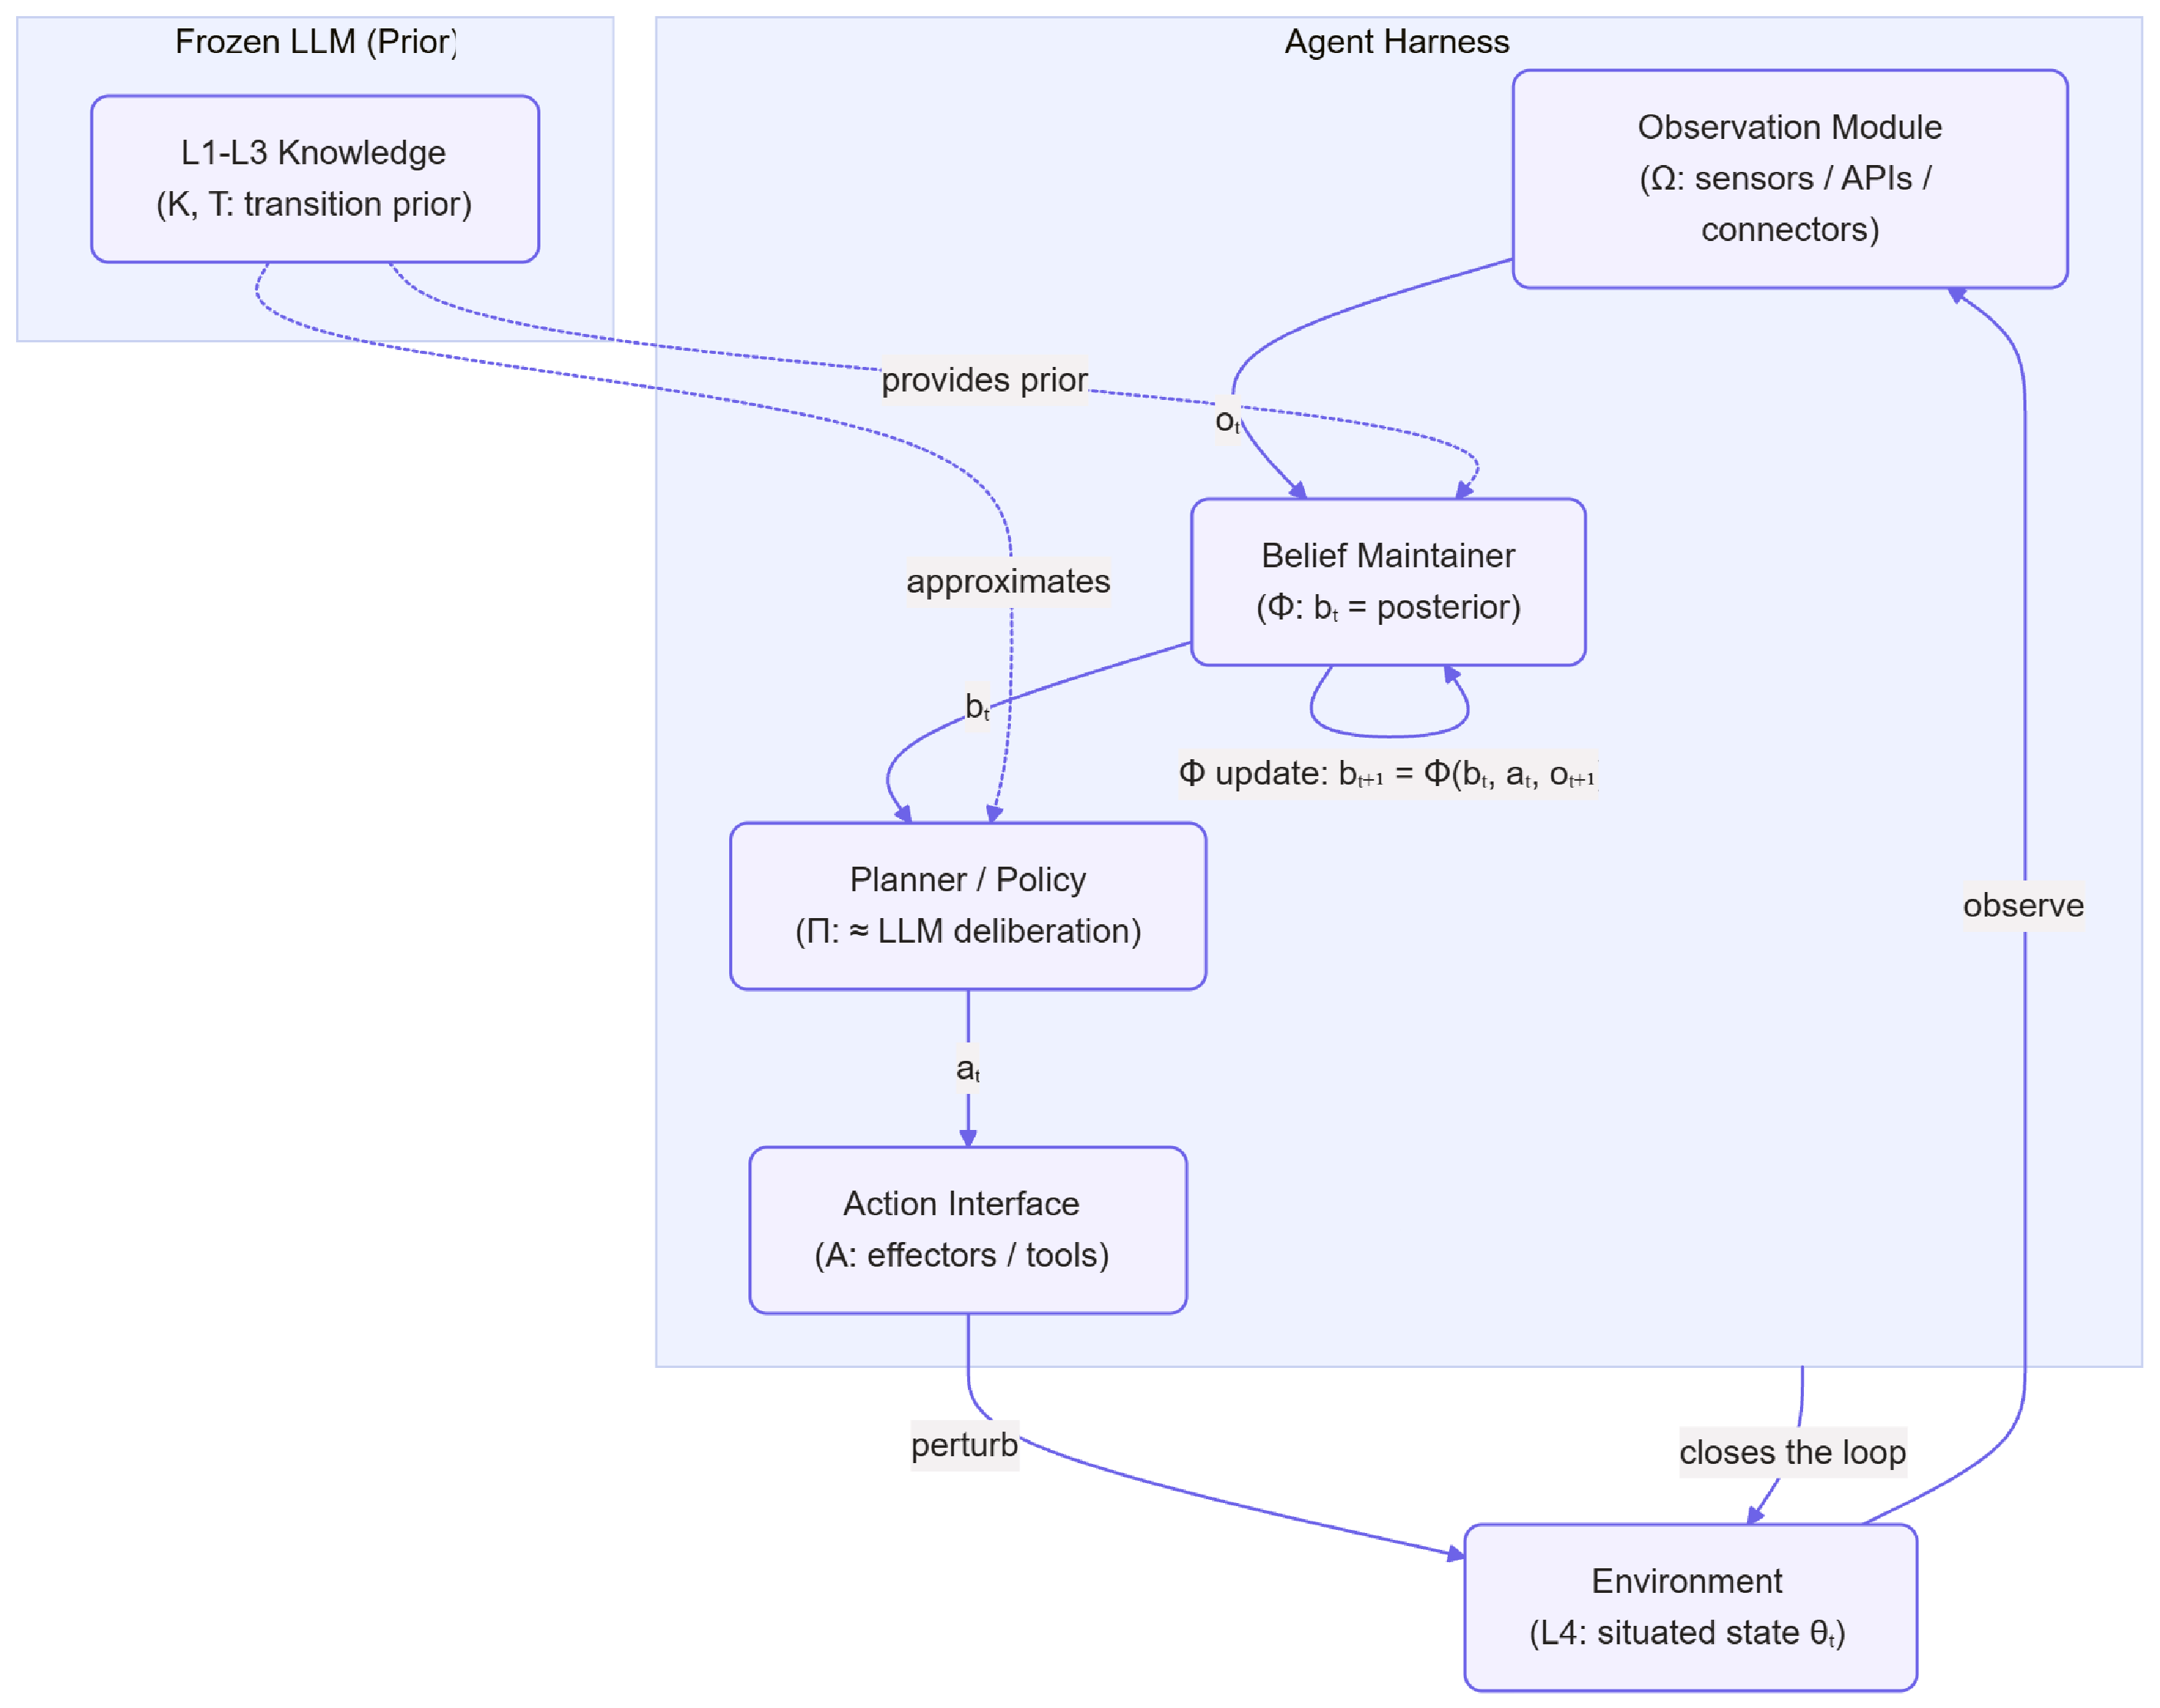
\includegraphics[width=0.85\textwidth]{figures/harness-architecture.pdf}
    \caption{The Agent Harness architecture. The frozen LLM provides \(\mathcal{K}\) and \(\mathcal{T}\); the Harness supplies \(\Omega\), \(\Phi\), and \(\Pi\). Solid arrows: data flow; dashed arrows: prior provision.}
    \label{fig:harness}
\end{figure*}
% 图：智能体框架架构。冻结LLM提供\(\mathcal{K}\)和\(\mathcal{T}\)；框架提供\(\Omega\)、\(\Phi\)和\(\Pi\)。实线箭头：数据流；虚线箭头：先验供给。

\subsection{Formalizing the Harness Architecture}

The Harness is a tuple:
\begin{equation}
\mathcal{H} = (\mathcal{S}, \mathcal{O}, \mathcal{A}, \mathcal{B}, \mathcal{T}, \Omega, \Pi),
\end{equation}
where each component corresponds to a concrete computational module:
% 框架定义为一个七元组，每个组件对应一个具体的计算模块：

\begin{itemize}
\item \(\mathcal{S} \subseteq \mathbb{R}^n\): the space of L4 environmental states \(\theta_t\), acted upon through effectors but not observed directly.
% \(\mathcal{S} \subseteq \mathbb{R}^n\)：L4环境状态\(\theta_t\)的空间，通过执行器作用于其上，但不直接观测。

\item \(\mathcal{O} \subseteq \mathbb{R}^m\): the observation space, comprising all possible observations \(o_t\) from observation modules.
% \(\mathcal{O} \subseteq \mathbb{R}^m\)：观测空间，包含来自观测模块的所有可能观测\(o_t\)。

\item \(\mathcal{A} \subseteq \mathbb{R}^k\): the action space available to the agent, instantiated through effectors.
% \(\mathcal{A} \subseteq \mathbb{R}^k\)：智能体可用的动作空间，通过执行器实例化。

\item \(\mathcal{B} \subseteq \Delta(\mathcal{S})\): the belief space, where \(b_t(\theta) = p(\theta_t \mid o_{1:t}, a_{1:t-1}, \mathcal{K})\) is the maintained posterior over L4 states.
% \(\mathcal{B} \subseteq \Delta(\mathcal{S})\)：信念空间，其中\(b_t(\theta) = p(\theta_t \mid o_{1:t}, a_{1:t-1}, \mathcal{K})\)是维护的L4状态后验。

\item \(\mathcal{T}: \mathcal{S} \times \mathcal{A} \to \Delta(\mathcal{S})\): the transition kernel
\begin{equation}
\mathcal{T}(\theta_{t+1} \mid \theta_t, a_t) = p(\theta_{t+1} \mid \theta_t, a_t, \mathcal{K}),
\end{equation}
representing the LLM's learned prior over dynamics.
% \(\mathcal{T}: \mathcal{S} \times \mathcal{A} \to \Delta(\mathcal{S})\)：转移核，表示LLM学习的动态先验。

\item \(\Omega: \mathcal{S} \to \Delta(\mathcal{O})\): the observation likelihood
\begin{equation}
\Omega(o_t \mid \theta_t) = \tilde{p}(o_t \mid \theta_t),
\end{equation}
implemented by external observation modules that transduce L4 states into textual observations.
% \(\Omega: \mathcal{S} \to \Delta(\mathcal{O})\)：观测似然，由外部观测模块实现，将L4状态转换为文本观测。

\item \(\Pi: \mathcal{B} \times \mathcal{G} \to \Delta(\mathcal{A})\): the policy/planner
\begin{equation}
\Pi(b_t, G) \approx \arg\min_{a \in \mathcal{A}} \mathbb{E}_{b_t}[\mathcal{C}(\theta, a) + \gamma V(b_{t+1})],
\end{equation}
approximated by the LLM through iterative deliberation, where \(\mathcal{G}\) is the goal space and \(\mathcal{C}\) encodes task and safety constraints.
% \(\Pi: \mathcal{B} \times \mathcal{G} \to \Delta(\mathcal{A})\)：策略/规划器，由LLM通过迭代推理近似，其中\(\mathcal{G}\)为目标空间，\(\mathcal{C}\)编码任务和安全约束。
\end{itemize}

Crucially, \(\Omega\) is not implemented by the LLM's parameters. It is supplied by external modules---sensors, APIs, or connectors---that transduce L4 into text. The grounding gap is structurally bounded by the fidelity of \(\Omega\), a constraint that scaling cannot alleviate.
% 关键在于，\(\Omega\)并非由LLM的参数实现，而是由外部模块（传感器、API或连接器）提供，将L4转译为文本。落地鸿沟在结构上受\(\Omega\)的保真度约束，这是缩放所无法缓解的。

\subsection{The Closed-Loop Dynamics}

The Harness operates as a discrete-time belief-state transition. The LLM provides \(\mathcal{T}\) and approximates \(\Pi\). But the posterior \(b_t(\theta)\) cannot be formed without \(\Omega\) and the recursive belief update \(\Phi\).
% 框架以离散时间信念状态转移的方式运作。LLM提供\(\mathcal{T}\)并近似\(\Pi\)。但后验\(b_t(\theta)\)缺少\(\Omega\)和递归信念更新\(\Phi\)则无法形成。

The loop operates in three stages:
% 环路分三个阶段运作：

\begin{enumerate}
\item \emph{Observation}: senses \(\theta_t\) and produces \(o_t\), implementing \(\Omega(o_t \mid \theta_t)\).
% \emph{观测}：感知\(\theta_t\)并产生\(o_t\)，实现\(\Omega(o_t \mid \theta_t)\)。

\item \emph{Belief update}: applies the Bayes filter \(\Phi\):
\begin{equation}
\begin{split}
b_{t+1} &= \Phi(b_t, a_t, o_{t+1}), \\
\Phi(b_t, a_t, o_{t+1})(\theta) &\propto \Omega(o_{t+1} \mid \theta) \\
&\quad \times \int_{\mathcal{S}} \mathcal{T}(\theta \mid \theta', a_t) \, b_t(\theta') \, d\theta'.
\end{split}
\end{equation}
% \emph{信念更新}：应用贝叶斯滤波器\(\Phi\)。后验正比于观测似然与预测信念的乘积。

\item \emph{Planning \& execution}: queries the LLM for \(\Pi(b_t, G)\) to produce \(a_t\), applies it via effectors, observes \(o_{t+1}\), and feeds back, closing \(b_t \to a_t \to o_{t+1} \to b_{t+1}\).
% \emph{规划与执行}：查询LLM获得\(\Pi(b_t, G)\)产生\(a_t\)，通过执行器施加，观测\(o_{t+1}\)并反馈，闭合环路\(b_t \to a_t \to o_{t+1} \to b_{t+1}\)。
\end{enumerate}

The Harness \emph{enacts} grounding, not merely accelerates it. Grounding is emergent from the coupled system.
% 框架\emph{施行}落地而非仅\emph{加速}落地。落地是耦合系统的涌现属性。

\subsection{The Harness as a Diagnostic Framework}

The tuple \(\mathcal{H}\) provides a precise vocabulary for diagnosing any LLM-based agent. For any system, we ask:
% 七元组\(\mathcal{H}\)为诊断任何基于LLM的智能体提供了精确术语。对于任何系统，我们问：

\begin{itemize}
\item Does it implement \(\Omega\) with sufficient fidelity \(\| \tilde{p} - p_{\text{real}} \|\) to track L4 dynamics?
% 是否以足够保真度\(\| \tilde{p} - p_{\text{real}} \|\)实现了\(\Omega\)以追踪L4动态？

\item Does it maintain \(b_t\) as a structured belief state updated via \(\Phi\) after each observation?
% 是否将\(b_t\)维护为通过\(\Phi\)在每次观测后更新的结构化信念状态？

\item Does it approximate \(\Pi\) using the LLM's offline knowledge and execute \(a_t\) through a causal interface?
% 是否利用LLM的离线知识近似\(\Pi\)并通过因果接口执行\(a_t\)？
\end{itemize}

L1--L3 coverage is evidenced by syntactic, physical, and factual reasoning---most current agents pass. L4 coverage, however, is evidenced only by the presence and fidelity of \(\Omega\) and \(\Phi\). By this measure, current systems cover L4 poorly, explaining their brittleness. Progress requires better Harnesses, not just better LLMs.
% L1-L3覆盖由句法、物理和事实推理证明——大多数当前智能体能通过。但L4覆盖只能由\(\Omega\)和\(\Phi\)的存在及其保真度证明。按此标准，当前系统对L4覆盖薄弱，这解释了它们的脆弱性。进步需要更好的框架，而不仅仅是更好的LLM。

The architecture is domain-general. For discrete L4 domains (e.g., DOM trees), the same framework applies with \(\mathcal{S}\) re-interpreted as a discrete state space. Two instantiations illustrate:
% 该架构是领域通用的。对于离散L4领域（如DOM树），同一框架在将\(\mathcal{S}\)重新解释为离散状态空间后仍然适用。两种实例化说明：

\begin{itemize}
\item \textbf{Physical agent} (robotics): \(\Omega\): cameras, LIDAR; \(\mathcal{A}\): motors, grippers. L4: positions, forces, occlusions.
% \textbf{物理智能体}（机器人）：\(\Omega\)：相机、激光雷达；\(\mathcal{A}\)：电机、夹爪。L4：位置、力、遮挡。

\item \textbf{Digital agent} (browser automation): \(\Omega\): DOM APIs, screenshot parsing; \(\mathcal{A}\): click, type, navigate. L4: DOM structure, application state.
% \textbf{数字智能体}（浏览器自动化）：\(\Omega\)：DOM API、截图解析；\(\mathcal{A}\)：点击、输入、导航。L4：DOM结构、应用状态。
\end{itemize}

In each case, the LLM provides \(\mathcal{T}\) and approximates \(\Pi\); the Harness supplies domain-specific \(\Omega\) and execution. The grounding problem is structurally identical across domains.
% 在每种情况下，LLM提供\(\mathcal{T}\)并近似\(\Pi\)；框架提供领域特定的\(\Omega\)和执行。落地问题在不同领域间结构上相同。

\subsection{Empirical Validation}

We instantiate the Harness on a code agent benchmark (158 EDA scripting tasks requiring correct pyAether API calls) to test our central claim: grounding gains come from \(\Omega\) fidelity, not model scale. We fix the LLM (DeepSeek-V4) and vary only the observation channel. Low-fidelity \(\Omega_{\text{vec}}\) uses name-only embedding; high-fidelity \(\Omega_{\text{hybrid}}\) combines name embedding, BM25 over descriptions, abbreviation expansion, and synonym redirect.
% 我们在一项代码智能体基准测试（158个EDA脚本任务，要求正确调用pyAether API）上实例化了该框架，以检验核心主张：落地增益来自\(\Omega\)保真度而非模型规模。固定LLM（DeepSeek-V4），仅改变观测通道。低保真\(\Omega_{\text{vec}}\)仅使用名称嵌入；高保真\(\Omega_{\text{hybrid}}\)结合名称嵌入、描述BM25、缩写展开和同义词重定向。

\begin{table*}[t]
\centering
\caption{Pass rate on 158 EDA tasks with fixed LLM, varying \(\Omega\) fidelity.}
\label{tab:omega}
\begin{tabular}{lcc}
\toprule
Configuration & \(\Omega\) Fidelity & Pass Rate \\
\midrule
Static prior only (no \(\Omega\)) & \(\varnothing\) & 0.0\% \\
Low-fidelity \(\Omega_{\text{vec}}\) & name-only & 59.5\% \\
High-fidelity \(\Omega_{\text{hybrid}}\) & name + desc + BM25 + abbrev & 87.3\% \\
\bottomrule
\end{tabular}
\end{table*}
% 表：158个EDA任务通过率，固定LLM，变化\(\Omega\)保真度。

Table~\ref{tab:omega} shows the results. With no runtime observation, pass rate is 0\%. With \(\Omega_{\text{vec}}\), it reaches 59.5\%. With \(\Omega_{\text{hybrid}}\), it improves to 87.3\%---a 27.8 percentage point gain from observation design alone, with the LLM unchanged. Over 20 Harness iterations on this benchmark, pass rate evolved from 59.5\% to 91.1\% without any model change, supporting our claim that environmental adaptation is achieved through observation and action channel design, not parameter tuning.
% 表~\ref{tab:omega}展示了结果。无运行时观测时通过率为0\%。\(\Omega_{\text{vec}}\)下为59.5\%。\(\Omega_{\text{hybrid}}\)下提升至87.3\%——仅通过观测设计就获得27.8个百分点增益，LLM不变。在该基准上经过20多次框架迭代，通过率从59.5\%演进至91.1\%，未改变任何模型，支持了我们的主张：环境适应通过观测和动作通道设计实现，而非参数调优。

\subsection{Design Principles}

The formalization yields three architectural principles:
% 上述形式化产生三条架构原则：

\begin{enumerate}
\item \emph{Closed-loop necessity}: The observation-action loop must be continuous; \(\Phi\)'s update rate must exceed the characteristic timescale of L4 dynamics.
% \emph{闭环必要性}：观测-动作环路必须持续；\(\Phi\)的更新率必须超过L4动态的特征时间尺度。

\item \emph{Observation fidelity}: Minimize \(\| \tilde{p} - p_{\text{real}} \|\) by optimizing observation modules. Information lost in \(\Omega\) cannot be recovered by a larger LLM.
% \emph{观测保真度}：通过优化观测模块最小化\(\| \tilde{p} - p_{\text{real}} \|\)。\(\Omega\)中丢失的信息无法由更大的LLM恢复。

\item \emph{Belief maintenance}: Maintain \(b_t\) as a structured representation capturing uncertainty and history, enabling recovery from unexpected changes.
% \emph{信念维护}：将\(b_t\)维护为捕获不确定性和历史的结构化表征，使其能从意外变化中恢复。
\end{enumerate}